\chapter{Receiver calibration}\label{chap:calibration}

% **************************** Define Graphics Path **************************
\ifpdf
    \graphicspath{{calibration/figs/Raster/}{calibration/figs/PDF/}{calibration/figs/}}
\else
    \graphicspath{{calibration/figs/Vector/}{calibration/figs/}}
\fi


With a working instrument capable of taking measurements in the field, the next step towards detection of the 21-cm signature is calibration of the experimental apparatus. There are many forms of calibration from physical antenna or ground plane modifications to numerical post-processing methods such as correctional atmospheric modelling. The need for more accurate cosmic signal measurements against the cacophony of unwanted noise demands finer degrees of calibration through the development of novel methods. At the current technological aim of millikelvin-level calibration, minute differences in an instrument’s electrical properties can skew spectral measurements enough to hamper a cosmological detection. In the previous chapter, we detailed the system architecture designed to minimise these distortions. Here we present a procedure to calibrate out the remaining systematic effects. The task has encompassed decades of research starting in the 1950’s where \citet{bauer_rothe} and \citet{rothe_dahlke} introduced a wave formulation of noise to microwave systems\footnote{\citet{bauer_rothe} presented in English by \citet{penfield}.} before a mathematical prescription to eliminate these noise waves through the derivation of “noise wave parameters” was conceived by \citet{meys} in 1978. This method, which inspires many contemporary radiometric calibration procedures, relies on the relative differences between sequential measurements of known passive devices to divide out small-timescale variability through a method known as “Dicke switching”, named after famed astronomer Robert Dicke. This relative calibration was utilised into the late 2000’s when \citet{edges_limits} placed a lower limit on the duration of the reionisation epoch at $\Delta z < 0.06$. It was quickly understood that the extraction of further information from 21-cm experimentation required a more powerful calibration method and work commenced to reformulate the noise wave parameters under an “absolute” calibration procedure which offered a more comprehensive derivation by referencing all measurements to an absolute temperature scale as well as expanding compatibility with instruments of increasing bandwidth \citep{rogersCal}. It was this absolute calibration that was used in the 2018 EDGES measurement where the authors quote a 20 mK calibration accuracy \citep{edgesNature, edgesCal}.


% =========================================
\section{Historical calibration formalism}\label{sec:historic_cal}
In the original formulation by \citet{rogersCal}, a noise temperature measured by the antenna is modelled as the sky noise temperature $\T{sky}$ minus some portion of the measurement reflected back into the sky due to impedance mismatches,
\begin{equation}
    \T{ant} = \T{sky} \left( 1 - |\Gamma|^2 \right),
    \label{eqn:sky_noise_temp}
\end{equation}
where the reflected portion is dependent on the reflection coefficient at the reference plane defined by the $50\Omega$ connection between the antenna and receiver, $\Gamma$. Following the argument in \citep{rogersCal} using $\Gamma$ redefined through impedances, \cref{eqn:sky_noise_temp} can be expanded using VNA measurements of the antenna and receiver input
\begin{equation}
    \T{ant} = \T{sky} \left( 1 - |\Gam{ant}|^2 \right) |F|^2,
    \label{eqn:sky_noise_temp_extend}
\end{equation}
where
\begin{equation}
    F = \frac{\sqrt{1-|\Gam{rec}|^2}}{1-\Gam{ant}\Gam{rec}}.
    \label{eqn:f}
\end{equation}
Here $\Gam{ant}$ and $\Gam{rec}$ are the reflection coefficients of the antenna and receiver respectively and the complex factor $F$ represents the noise waves reflected back and forth between the antenna and receiver summed as a polylogarithmic series.

Additionally, noise from the LNA moving toward the receiver input and antenna is reflected and enters the signal chain as noise. Incorporating this into \cref{eqn:sky_noise_temp_extend} gives us the receiver noise temperature
\begin{equation}
    \T{rec} = \T{sky} \left( 1 - |\Gam{ant}|^2 \right) |F|^2 + \T{unc}|\Gam{ant}|^2|F|^2 + \left( \T{cos}\cos(\phi) + \T{sin}\sin(\phi) \right) |\Gam{ant}||F| + T_0,
    \label{eqn:trec}
\end{equation}
where $\T{unc}$ is the portion of the noise reflected by the antenna that is uncorrelated with the LNA output, $\T{cos}$ and $\T{sin}$ are the cosine and sine components of noise reflected by the antenna that \textit{are} correlated with the LNA, $\phi$ is the phase of the reflections equal to $\mathrm{arg}\left(\Gam{ant}F\right)$ and $T_0$ is the portion of noise independent of the LNA\footnote{$T_0$ is also referred to as the ‘receiver noise offset’ \citep{edgesCal}.} \citep{rogersCal}. \citet{rogersCal} note that \cref{eqn:trec} is equivalent to the noise wave formulation of \citet{meys}.

Through use of the three-position Dicke switch, the LNA is sequentially connected to the antenna, ambient $50\Omega$ load and the noise source recording the power at each position
\begin{equation}
    \psd{ant} = g \T{rec},
    \label{eqn:rogers_pant}
\end{equation}
\begin{equation}
    \psd{L} = g \left[  \left( 1 - |\Gam{rec}|^2 \right) \T{L} + T_0 \right],
    \label{eqn:rogers_pl}
\end{equation}
\begin{equation}
    \psd{NS} = g \left[ \left( 1 - |\Gam{rec}|^2 \right) \left( \T{L} + \T{NS} \right) + T_0 \right],
    \label{eqn:rogers_pns}
\end{equation}
representing the power measured at the antenna, reference load and reference noise source respectively. Here $\T{L}$ and $\T{NS}$ are the temperatures of the reference ambient-temperature load and noise source while $g$ is the receiver gain. In reality, \cref{eqn:rogers_pl} and \cref{eqn:rogers_pns} should have terms corresponding to $\T{unc}$, $\T{cos}$ and $\T{\sin}$ (as in \cref{eqn:rogers_pant} when expanded via \cref{eqn:trec}), but the low reflection coefficients of the reference load and noise source (< -40 dB) suggest $\Gam{L},\Gam{NS}\rightarrow0$ and are set as such in this formulation. The uncalibrated antenna temperature is then
\begin{equation}
    \T{ant}^* = \T{NS} \frac{\left( \psd{ant} - \psd{L} \right)}{\left( \psd{NS} - \psd{L} \right)} + \T{L},
    \label{eqn:tant_star}
\end{equation}
where all terms in the equation are frequency-dependent, though not explicitly shown for simplicity of notation. The quotient in \cref{eqn:tant_star} is used to remove short term variations in system gain and is referred to as the ‘q-term’ in EDGES-related presentations and publications \citep{murray_calpap},
\begin{equation}
    q =  \frac{\left( \psd{ant} - \psd{L} \right)}{\left( \psd{NS} - \psd{L} \right)}.
    \label{eqn:qterm}
\end{equation}
Plugging in the definitions for $\psd{ant}$, $\psd{L}$ and $\psd{NS}$ of \cref{eqn:rogers_pant,eqn:rogers_pl,eqn:rogers_pns} into \cref{eqn:tant_star} gives us our expanded form for the calibrated antenna temperature
\begin{equation}
    \T{ant}^* = \T{sky}\frac{\left(1 - |\Gam{ant}|^2\right)|F|^2}{1 - |\Gam{rec}|^2} + \T{unc}\frac{|\Gam{ant}|^2|F|^2}{1 - |\Gam{rec}|^2} + \left( \T{cos}\cos(\phi) + \T{sin}\sin(\phi) \right)\frac{|\Gam{ant}||F|}{1 - |\Gam{rec}|^2}.
    \label{eqn:rogers_calibrated_temp}
\end{equation}
In the EDGES formulation, the values for $\T{L}$ and $\T{NS}$ were approximated based on ‘realistic assumptions for the noise temperatures’ \citep{edgesCal} while the noise wave parameters $\T{unc}$, $\T{cos}$ and $\T{sin}$ were determined through measurements of the opened and shorted low-loss cables connected as calibration sources which again act as an antenna viewing an isotropic sky with temperature equal to the cables’ physical temperatures \citep{rogersCal}.

This methodology was further developed for the EDGES high-band receiver which was included in the controversial detection of an absorption profile centred at 78 MHz \citep{edgesNature}. In the updated form, the power spectral densities are expressed in terms of specific instrument response contributions similar to \cref{eqn:rogers_pant,eqn:rogers_pl,eqn:rogers_pns},
\begin{multline}
    \psd{ant} = g \Big[ \T{sky} \left( 1 - |\Gam{ant}|^2 \right) |F|^2 + \T{unc}|\Gam{ant}|^2|F|^2 + \T{cos}|\Gam{ant}||F|\cos(\phi) \\
    + \T{sin}|\Gam{ant}||F|\sin(\phi) + T_0 \Big],
    \label{eqn:pant}
\end{multline}
with $F$ defined as in \cref{eqn:f} and $\phi$ remaining as the reflection phase. Maintaining the assumption that the reference load and noise source have a negligible reflection coefficient, the corresponding power spectral densities follow \cref{eqn:rogers_pl,eqn:rogers_pns} where
\begin{equation}
    \psd{L} = g^* \left[ \T{L} \left( 1 - |\Gam{rec}|^2 \right) + T_0^* \right],
    \label{eqn:pl}
\end{equation}
\begin{equation}
    \psd{NS} = g^* \left[ \left( \T{L} + \T{NS} \right) \left( 1 - |\Gam{rec}|^2 \right) + T_0^* \right].
    \label{eqn:pns}
\end{equation}
Here, the system gain ($g^*$) and noise offset ($T_0^*$) are different from \cref{eqn:pant} as the internal reference devices are injected at a slightly different reference plane than the antenna at the receiver input (compare \citet{edgesCal} Figure 2 with \cref{fig:overview}). Due to this, EDGES introduces two corrective terms, $C_1$ and $C_2$, when expanding \cref{eqn:tant_star} yielding
\begin{multline}
    \left( \T{ant}^* - \T{L} \right)C_1 + \left( \T{L} - C_2 \right) = \T{sky}\left[ \frac{\left(1-|\Gam{ant}|^2\right)|F|^2}{1 - |\Gam{rec}|^2} \right] + \T{unc}\left[\frac{|\Gam{ant}|^2|F|^2}{1 - |\Gam{rec}|^2} \right] \\
    + \T{cos}\left[ \frac{|\Gam{ant}||F|}{1 - |\Gam{rec}|^2}\cos(\phi) \right] + \T{sin}\left[ \frac{|\Gam{ant}||F|}{1 - |\Gam{rec}|^2}\sin(\phi)\right].
    \label{eqn:edges_second_calibrated_temperature}
\end{multline}
Here $C_1$ and $C_2$ represent a scale and offset that collectively correct for the first-order approximations for $\T{L}$ and $\T{NS}$ as well as the differing reference planes between the receiver input and the input point of the internal reference sources and the reflection coefficients of the internal reference sources which were set to zero in \cref{eqn:pl} and \cref{eqn:pns} \citep{edgesCal}.

In the EDGES methodology, four calibrators are used to determine the noise wave parameters and offset terms; an ambient load, a heated load, an eight metre coaxial cable with an opened end and the same coaxial cable with a shorted end. With each of these calibration sources at the receiver input, the VNA measures the reflection coefficient of the calibrator and the receiver input for calculation of $F$ from \cref{eqn:f} and $\phi$, followed by spectrometer measurements of the power spectral densities at the input for calculation of the uncalibrated input temperature through \cref{eqn:tant_star} as well as the calibrators’ physical temperatures. With regard to the heated $50 \Omega$ load however, an extra step is needed to take into account the temperature gradient exhibited across the heated load construction (see \cref{fig:hot_load}). An effective noise temperature, $\T{ht}$, is derived through measurements of the physical temperature at the termination, $\T{term}$, and of the cable, $\T{cab}$
\begin{equation}
    \T{ht} = G\T{term} + \left( 1 - G \right) \T{cab}.
    \label{eqn:hot_load_correction}
\end{equation}
$G$ in this equation is the available power gain of the assembly which is defined in \citet{pozar}
\begin{equation}
    G = \frac{|S_{21}|^2 \left( 1 - |\Gam{term}|^2 \right)}{|1 - S_{11}\Gam{term}|^2 \left(1 - |\Gam{hot}|^2 \right)},
    \label{eqn:g}
\end{equation}
where $\Gam{hot}$ is the measured reflection coefficient of the heated load device as a whole, $\Gam{term}$ is the reflection coefficient of the termination from the heated load alone and $S_{11}$ and $S_{21}$ are the S-parameters of the cable used in the heated load construction. For these measurements, port 1 refers to the port attached to the termination and port 2 corresponds to the end connected to the receiver. For the EDGES experiment, all of the above quantities are measured in the laboratory before deployment to site \citep{edgesCal}. Two points that are relevant to our methodology is that EDGES integrates spectral measurements for 24 hours for each calibrator and that all reflection coefficients of the receiver input are measured with a VNA port power of -30 dBm to avoid letting the LNA saturate the device during measurements. The VNA itself is calibrated before every measurement as is done in our technique.

With all calibration measurements in place, the $C_1$ and $C_2$ terms are computed through an iterative approach (see \citet{edgesCal}) followed by a least squares fit of the noise wave parameters $\T{unc}$, $\T{cos}$ and $\T{sin}$ from the sets of \cref{eqn:edges_second_calibrated_temperature}’s afforded by the calibration source measurements minimising the difference between the uncalibrated input temperature $\T{ant}^* \rightarrow \T{cal}^*$ from \cref{eqn:tant_star} and the measured physical temperature of the calibrator as $\T{ant} \rightarrow \T{cal}$. The least squares procedures solves for the calibration parameters as order-seven polynomials in frequency with the parameters taking the approximate values of 0.9 for $C_1$, $-6$ for $C_2$, 67 K for $\T{unc}$, -20 K for $\T{cos}$ and 10 K for $\T{sin}$ \citep{edgesCal}. The calibration accuracy of the method is reported to be 26 mK \citep{edgesCal}.


% =========================================
\section{Reformulation for \textsc{Excalibrate}}\label{sec:reach_formalism}
 In response to the controversy surrounding the EDGES experiment, we have strived to improve the methodology and address discrepancies in the procedure through the introduction of a Bayesian calibration framework which we formulate over the following sections. The noise necessitating calibration arises during measurements. For a global experiment, we measure a sky temperature $\T{sky}(\Omega, \nu, t)$ as a function of the direction $\Omega$, frequency $\nu$ and time $t$ which can be broken down into two primary components: the global 21-cm signal $T_{21}$ and astrophysical foregrounds $\T{f}$
\begin{equation}
    \label{tsky}
    \T{sky}(\Omega, \nu, t) = T_{21}(\nu) + \T{f}(\Omega, \nu, t).
\end{equation}
Sky signals absorbed by the antenna convolve with the normalised antenna directivity $B$, introducing systematic noise represented by our random noise term $N_{\mathrm{data}}$.
\begin{equation}\label{eqn:bayestsource}
    D(\nu, t) = \int \T{sky}(\Omega, \nu, t) B(\Omega, \nu)\mathrm{d}\Omega + N_{\mathrm{data}}.
\end{equation}
Thus, our 21-cm signature can be formulated as
\begin{equation}\label{signal}
  T_{21} \approx D(\nu, t) - \int\T{f}(\Omega, \nu, t)B(\Omega, \nu)\mathrm{d}\Omega - N_{\mathrm{data}}.
\end{equation}
A diagram illustrating the evolution of the sky signal during this process in shown in \cref{fig:nsfig}.
\begin{figure}
    \centering
    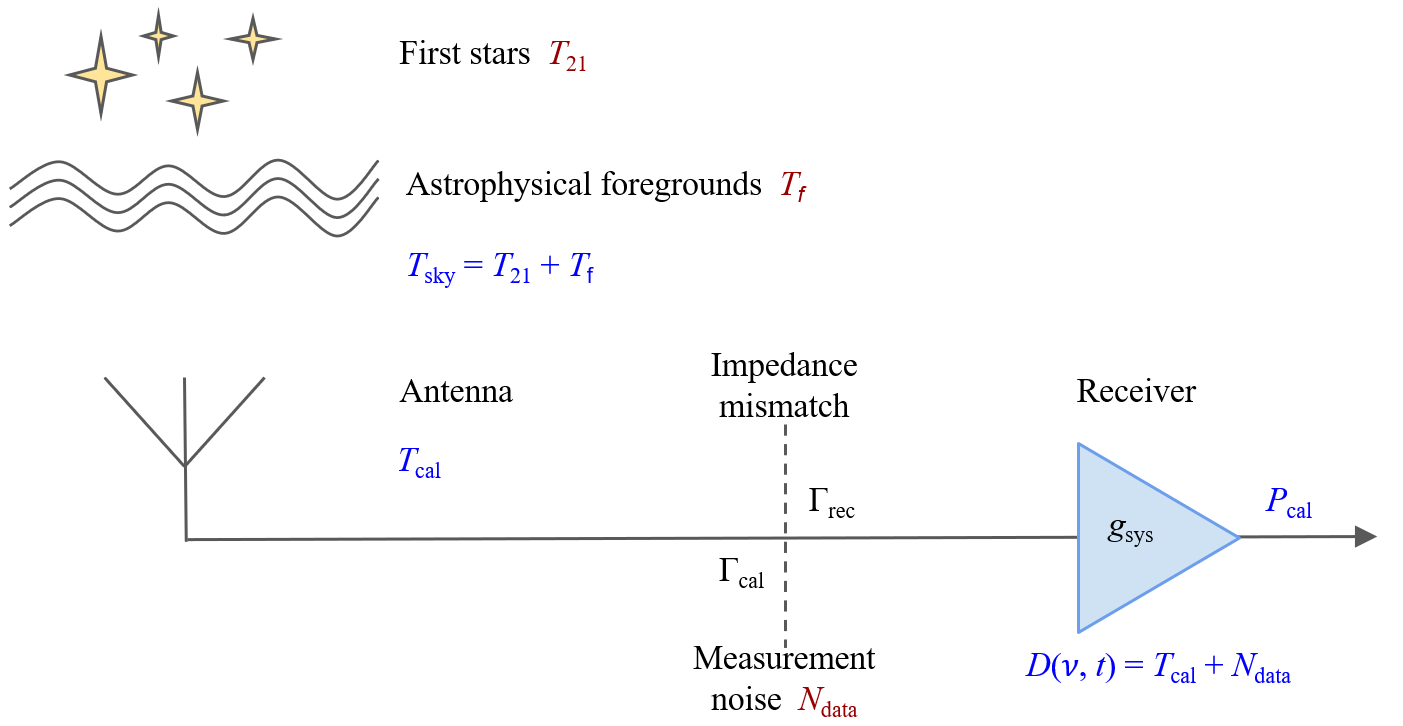
\includegraphics[width=.7\textwidth]{nsdiag}
    \caption{Diagram showing the evolution of the 21-cm signal hampered by astrophysical foregrounds, convolvution with the antenna beam and the emergence of measurement noise before calibration to retrieve the sky temperature.}
    \label{fig:nsfig}
\end{figure}
The integral in \cref{signal} is assessed through foreground and beam modelling techniques such as those discussed in \citet{dom} while modelling of $N_{\mathrm{data}}$ from the (statistical) properties of $D(\nu, t)$ is accomplished through calibration.

The framework for \textsc{Excalibrate} follows the Dicke switching strategy used by EDGES \citep{edgesCal} and LOFAR \citep{lofarCal} in much the same way with power spectral densities of calibration sources and internal references used to calculate an uncalibrated input temperature according to \cref{eqn:tant_star}. We however have reformulated the power spectral densities in terms of the specific response contributions
\begin{multline}
    \label{eqn:reach_pant}
    \psd{cal} = g_{\mathrm{sys}} \Bigg[ \T{cal}\left(1-|\Ga|^2\right)\left|\frac{\sqrt{1 - |\Gam{rec}|^2}}{1-\Ga\Gam{rec}}\right|^2 + \T{unc}|\Ga|^2\left|\frac{\sqrt{1 - |\Gam{rec}|^2}}{1-\Ga\Gam{rec}}\right|^2 \\
    + \T{cos}\operatorname{Re}\left(\Ga\frac{\sqrt{1 - |\Gam{rec}|^2}}{1-\Ga\Gam{rec}}\right) + \T{sin}\operatorname{Im}\left(\Ga\frac{\sqrt{1 - |\Gam{rec}|^2}}{1-\Ga\Gam{rec}}\right) + T_0 \Bigg],
\end{multline}
where $\psd{cal}$, $\Gam{cal}$ and $\T{cal}$ are the power spectral density, reflection coefficient and measured temperature of the calibratrion source under test at the receiver input. $g_{\mathrm{sys}}$ is the system gain referenced to the receiver input. Additionally, the phase terms accompanying $\T{cos}$ and $\T{sin}$ in \cref{eqn:pant} are now described by the Re() and Im() arguments which are equivalent to $\phi$ in the EDGES notation \cite{rogersCal}.

Similar assumptions of negligible reflection coefficients for the internal references as well as an independent reference plane for these devices (once again, see \cref{fig:overview}) allow for $\psd{L}$ and $\psd{NS}$ to remain the same as \cref{eqn:pl} and \cref{eqn:pns}. Expanding \cref{eqn:tant_star} using \cref{eqn:reach_pant,eqn:pl,eqn:pns} yields our version of the linear relationship between the uncalibrated input temperature and a final calibrated temperature of any device connected to the receiver input
\begin{multline}
    \label{eqn:caleqn}
    \T{NS}\left( \frac{\psd{cal} - \psd{L}}{\psd{NS} - \psd{L}} \right) + \T{L} = \T{cal}\left[ \frac{1-|\Ga|^2}{|1-\Ga\Gam{rec}|^2} \right] + \T{unc}\left[ \frac{|\Ga|^2}{|1-\Ga\Gam{rec}|^2} \right] \\
    + \T{cos}\left[ \frac{\operatorname{Re}\left(\frac{\Ga}{1-\Ga\Gam{rec}}\right)}{\sqrt{1-|\Gam{rec}|^2}} \right] + \T{sin}\left[ \frac{\operatorname{Im}\left(\frac{\Ga}{1-\Ga\Gam{rec}}\right)}{\sqrt{1-|\Gam{rec}|^2}} \right].
\end{multline}
We note that our reformulation solves for $\T{L}$ and $\T{NS}$ as parameters directly rather than using the corrective $C$ factors of the EDGES procedure. Some advantages to our approach are that all parameters to be solved for are now in units of temperature as well as the verifiability of the $\T{L}$ and $\T{NS}$ parameters through comparison with thermocouple readings and manufacturer specifications (compare \cref{fig:ns_diode} with \cref{fig:ls_nwps}) respectively. 

We will now simpify the notation of our approach by defining the following terms;
\begin{equation}\label{eqn:xunc}
    X_{\mathrm{unc}} = -\frac{|\Ga|^2}{ 1-|\Ga|^2}, 
\end{equation}
\begin{equation}\label{eqn:xl}
    X_{\mathrm{L}} = \frac{|1-\Ga\Gr|^2}{1-|\Ga|^2},
\end{equation}
\begin{equation}\label{eqn:xcos}
    X_{\mathrm{cos}} = -\operatorname{Re}\left(\frac{\Ga}{1-\Ga\Gr} \times \frac{X_{\mathrm{L}}}{\sqrt{1-|\Gr|^2}}\right),
\end{equation}
\begin{equation}\label{eqn:xsin}
    X_{\mathrm{sin}} = -\operatorname{Im}\left(\frac{\Ga}{1-\Ga\Gr} \times \frac{X_{\mathrm{L}}}{\sqrt{1-|\Gr|^2}}\right),
\end{equation}
\begin{equation}\label{eqn:xns}
    X_{\mathrm{NS}} = \left( \frac{P_{\mathrm{cal}}-P_{\mathrm{L}}}{P_{\mathrm{NS}}-P_{\mathrm{L}}} \right) X_{\mathrm{L}},
\end{equation}
which represent initial calibration measurements on $D$ in the frequency domain for the characterisation of $N_{\mathrm{data}}$ from \cref{eqn:bayestsource} via our noise wave parameters. Here we assume that calibration-related deviations of $D$ on the timescale of a single calibration-observation run are sufficiently curtailed through practical strategies such as temperature control of the receiver environment. Incorporating these equations into \cref{eqn:caleqn}, with some rearrangement, then gives
\begin{equation}
    X_{\mathrm{unc}}\T{unc} + X_{\mathrm{cos}}\T{cos} + X_{\mathrm{sin}}\T{sin} + X_{\mathrm{NS}}\T{NS} + X_{\mathrm{L}}\T{L} = \T{cal},
    \label{eqn:almost_expanded_cal_eqn}
\end{equation}
at each frequency. We can see here that there are no squared or higher-order terms, allowing us to take advantage of the linear form by grouping the data and noise wave parameters into separate matrices
\begin{equation} \label{eqn:theta}
    \begin{split}
    \mathbfss{X} &\equiv \begin{pmatrix} 
        X_\mathrm{unc} \quad 
        X_\mathrm{cos} \quad
        X_\mathrm{sin} \quad
        X_\mathrm{NS} \quad
        X_\mathrm{L} \end{pmatrix}, \\
    \boldsymbol{\Theta} &\equiv \begin{pmatrix} 
        T_\mathrm{unc}\quad
        T_\mathrm{cos}\quad
        T_\mathrm{sin}\quad
        T_\mathrm{NS}\quad
        T_\mathrm{L}\end{pmatrix}^\top.
    \end{split}
\end{equation}

Under this formulation, all of our data; the reflection coefficient measurements and power spectral densities, are grouped in an $\mathbfss{X}$ vector which forms a matrix with axes of data by frequency. The calibration parameters as frequency-dependent polynomials of varying degree are collected into a $\boldsymbol{\Theta}$ vector which serves as our model describing $N_{\mathrm{data}}$. Applying the definitions of \cref{eqn:theta} to \cref{eqn:almost_expanded_cal_eqn} condenses the calibration equation into
\begin{equation}\label{eqn:linearmodel}
    \y = \mathbfss{X}\boldsymbol{\Theta}+\sigma,
\end{equation}
where $\y$ is a vector over frequency and $\sigma$ is a noise vector representing our error. Since EDGES assumes that each power spectral density measurement is frequency independent, we have assumed that $\sigma$ is a multivariate normal distribution. This assumption is implicit in the EDGES analysis in which they use a least-squares minimisation approach for solving model parameters.


% =========================================
\section{A Bayesian approach}\label{sec:bayes}
From an instrumentation perspective, a possible source of the systematics thought to affect the EDGES measurement is the calibration of their instrument in a controlled laboratory setting separate from the environment in which astrophysical observations take place. At the milli-kelvin level, these environmental effects may be non trivial. Parameters related to the physical instrument are expected to change such as the antenna response due to heat expansion or impedance fluctuations of delicate front-end components. As corroborated by the various experiments in \cref{sec:responses}, this may especially be the case with regards to how the calibration parameters change between observation runs. Furthermore, the fixed seven-term polynomial used by EDGES to model all of their noise wave parameters may underfit or overfit individual parameters and thus `fit out' data useful for determining systematics or potentially even the 21-cm signal itself if a joint fit is performed.

In response to these concerns, we have developed a calibration pipeline that improves on the strategies presented in \citet{edgesCal} and introduce a novel Bayesian methodology using conjugate priors, allowing for a dynamic application of our algorithm in the field with astrophysical data collection regardless of system complexity. Also included are model selection procedures for the optimisation of  individual noise wave parameters to combat overfitting and underfitting, the results of which converge with that of a least-squares approach when wide priors are adopted. Our pipeline easily incorporates many more calibration sources than the standard four as shown in \cref{sec:frontend} for increased constraints on noise wave parameters while identifying possible correlations between parameters. A schematic overview of our improved Bayesian calibration method is shown in \cref{fig:cal_flowchart}.
\begin{figure}
    \centering
    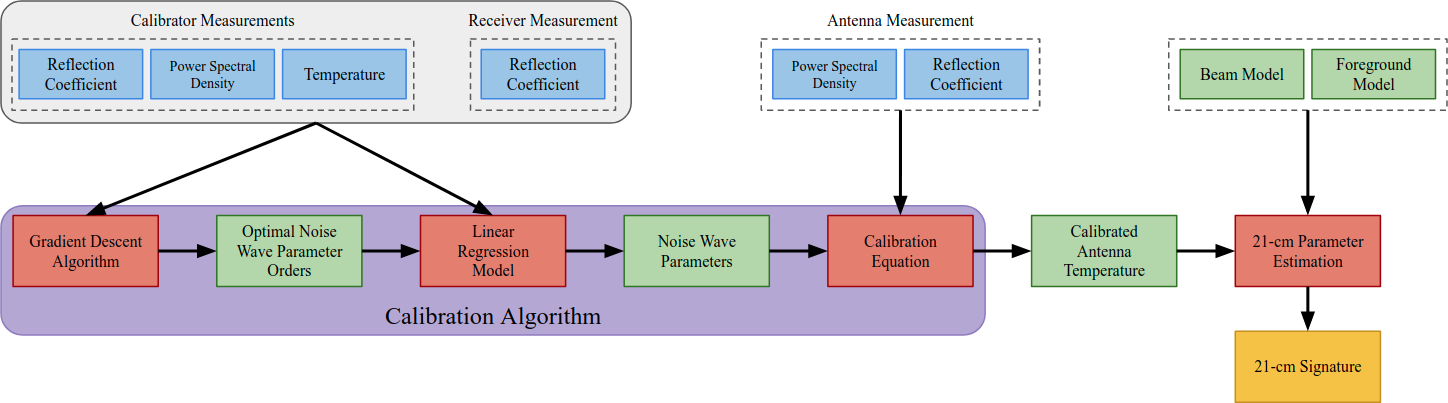
\includegraphics[width=\textwidth]{cal_flowchart}
    \caption{Outline of our Bayesian calibration algorithm. Blue blocks represent data to be taken, red blocks represent calculations and green blocks represent calculation outputs.}
    \label{fig:cal_flowchart}
\end{figure}

To start we briefly review the Bayesian methodology used to quantify logical reasoning. In the representation of relative beliefs in the validity of multiple propositions, it is natural to assign real numbers to propositions with larger numerical values corresponding to greater belief in a proposal. Under the constraint that identical information should lead to identical conclusions, we find that this approach is only consistent if the numerical values assigned to our beliefs in various propositions obey probability theory, including the product rule describing conditional probability \citep{sivia_skilling}
\begin{equation}
    \mathrm{prob}(X,Y|I) = \mathrm{prob}(X|Y,I) \times \mathrm{prob}(Y|I),
    \label{eqn:productrule}
\end{equation}
which simply represents the notion that given some background information $I$, the probability that the propositions $X$ and $Y$ are both true is equal to the probability that $X$ is true given that $Y$ is true times the probability that $Y$ is true. A transposition of \cref{eqn:productrule} gives
\begin{equation}
    \mathrm{prob}(Y,X|I) = \mathrm{prob}(Y|X,I) \times \mathrm{prob}(X|I),
    \label{eqn:product_transpose}
\end{equation}
which states the transpose of \cref{eqn:productrule}; the probability that $Y$ and $X$ are both true is equal to the probabiility that $Y$ is true given $X$ times the probability that $X$ is true. Adhering to the assertion that identical information leads to identical conclusions, the statement ‘both $X$ and $Y$ are true’ must be equivalent to the statement ‘both $Y$ and $X$ are true’ and we can thus equate \cref{eqn:productrule} and \cref{eqn:product_transpose} which, with some rearrangement, reveals Bayes' Theorem:
\begin{equation}
    \mathrm{prob}(X|Y,I) = \frac{\mathrm{prob}(Y|X,I) \times \mathrm{prob}(X|I)}{\mathrm{prob}(Y|I)}.
    \label{eqn:bayes}
\end{equation}
This equation is the foundation for Bayesian statistics and relates the probability that a model $X$ is true given data $Y$ and background information $I$ to a quoteint of three probability distributions. The first quantity in the numerator of \cref{eqn:bayes}, $\mathrm{prob}(X|I)$ is our ‘prior’ probability representing any prior knowledge before analysis of the data. In the light of data from experimental measurements, the likelihood function $\mathrm{prob}(Y|X,I)$ updates our prior distribution to a ‘posterior’ probability $\mathrm{prob}(X|Y,I)$ which represents our belief in the hypothesis after taking the data into account. The denominator of \cref{eqn:bayes} is a normalisation constant known as the ‘evidence’. When evaluating competing models such as plausible but independent sets of calibration parameter values, comparison of the evidence will determine the model preferred by the data (through the notion that a more likely proposal will have a larger numerical value). This will allow us to estimate the calibration parameters through the evaluation of competing models for the one that maximises the evidence.


% =========================================
\subsection{Specifying our probability distributions}
\label{sec:likelihood}
For calibration of the receiver, we are concerned with the construction of predictive models of the noise wave parameters, $\boldsymbol{\Theta}$, in the context of some dataset, $\mathbfit{T}$. We can use $\boldsymbol{\Theta}$ to calculate the probability of observing the data given a specific set of noise wave parameters:
\begin{equation}\label{likelihood}
    p\big(\mathbfit{T} \given[\big] \boldsymbol{\Theta}, \sigma^2\big) = \frac{1}{2\pi \sigma^2}^{N/2}\exp{ \Bigg\{ -\frac{1}{2\sigma^2}\left(\mathbfit{T}-\mathbfss{X}\boldsymbol{\Theta}\right)^{\top}\left(\mathbfit{T} -\mathbfss{X}\boldsymbol{\Theta}\right) \Bigg\}},
\end{equation}
where, $N$ is the number of measurements. This distribution on the data is our likelihood. For the purposes of calibration, $\mathbfit{T}$ may be $\y$ measurements or alternatively, $\mathbfit{T}_{\mathrm{sky}}$ for prediction of a sky signal. Our model must also specify a prior distribution, quantifying our initial assumptions on the values and spread of our noise wave parameters which we specify as a multivariate normal inverse gamma distribution:
\begin{equation}
  \label{eqn:prior}
  p\left(\boldsymbol{\Theta}, \sigma^2\right) \propto \left(\frac{1}{\sigma^2}\right)^{a+1+\left(d/2\right)} \times \exp \left[ -\frac{1}{\sigma^2}\{b+\frac{1}{2}\left(\boldsymbol{\Theta}-\boldsymbol{\mu}_{\boldsymbol{\Theta}}\right)^{\top}\mathbfss{V}_{\boldsymbol{\Theta}}^{-1}\left(\boldsymbol{\Theta}-\boldsymbol{\mu}_{\boldsymbol{\Theta}}\right)\} \right].
\end{equation}
Here, $a$ and $b$, which are greater than zero, along with $\mathbfss{V}_{\boldsymbol{\Theta}}$ and $\boldsymbol{\mu}_{\boldsymbol{\Theta}}$ represent our prior knowledge on the noise wave parameters. $d$ is the length of our vector $\boldsymbol{\Theta}$.

\Cref{likelihood} is determined by a set of values for our model $\boldsymbol{\Theta}$. We can marginalise out the dependence on $\boldsymbol{\Theta}$ and our noise term by integrating over the prior distribution by both $\boldsymbol{\Theta}$ and $\sigma^2$ at once. Following the steps in \citet{banerjee}
\begin{equation}
    \begin{aligned} \label{eqn:ev}
    p\left(\y\right) &= \int p\left(\y \given[\big] \boldsymbol{\Theta}, \sigma^2\right) p\left(\boldsymbol{\Theta}, \sigma^2\right) \mathrm{d}\boldsymbol{\Theta} \mathrm{d}\sigma^2,\\
    &= \frac{b^a\Gamma\left(a^*\right)\sqrt{|\mathbfss{V}^*|}}{{b^*}^{a^*}\Gamma\left(a\right)\sqrt{|\mathbfss{V}_{\boldsymbol{\Theta}}|}}(2\pi)^{-N/2}, \\
    \end{aligned}
\end{equation}
where 
\begin{equation}\label{starred}
    \begin{aligned}   
    a^* &= a + \frac{N}{2}, \\
    b^* &= b + \frac{1}{2}[\boldsymbol{\mu}_{\boldsymbol{\Theta}}^{\top}\mathbfss{V}_{\boldsymbol{\Theta}}^{-1}\boldsymbol{\mu}_{\boldsymbol{\Theta}} + \y^{\top}\y - \boldsymbol{\mu}^{*\top}\mathbfss{V}^{*-1}\boldsymbol{\mu}^*], \\
    \boldsymbol{\mu}^* &= \left(\mathbfss{V}_{\boldsymbol{\Theta}}^{-1} + \mathbfss{X}^{\top}\mathbfss{X}\right)^{-1}\left(\mathbfss{V}_{\boldsymbol{\Theta}}^{-1}\boldsymbol{\mu}_{\boldsymbol{\Theta}} + \mathbfss{X}^{\top}\y\right), \\
    \mathbfss{V}^* &= \left(\mathbfss{V}_{\boldsymbol{\Theta}}^{-1} + \mathbfss{X}^{\top}\mathbfss{X}\right)^{-1}, \\
    \end{aligned}
\end{equation}
and $\Gamma\left(x\right)$ represents the Gamma function, not to be confused with the notation for our reflection coefficients. \Cref{eqn:ev} is our evidence, which gives the probability of observing the data $\y$ given our model.\footnote{It is in fact better to use the equivalent more numerically stable expression
$b^*=b + \boldsymbol{q}^{\top} \boldsymbol{q} + \boldsymbol{q}^{\top} \mathbfss{X} \mathbfss{V}_{\boldsymbol{\Theta}} \mathbfss{X}^{\top} \boldsymbol{q}$,  where $\boldsymbol{q}= \y-\mathbfss{X}\boldsymbol{\mu}^*$ to avoid cancellation of large terms.}

With the prior distribution specified, we use Bayes' equation to invert the conditioning of the likelihood and find the posterior using the likelihood, prior and evidence:
\begin{equation}
    p\left(\boldsymbol{\Theta}, \sigma^2 \given[\big] \y\right) = \frac{p\left(\y \given[\big]  \boldsymbol{\Theta}, \sigma^2\right)p\left(\boldsymbol{\Theta}, \sigma^2\right)}{p\left(\y\right)}.
\end{equation}
Similarly from \citet{banerjee}, this can be written as
\begin{equation}
    \label{eqn:post}
    p\Bigl(\boldsymbol{\Theta},\sigma^2 \given[\big] \y\Bigl) \propto \left(\frac{1}{\sigma^2}\right)^{a^* + \frac{d}{2} + 1} \times \exp{ \Bigg\{ -\frac{1}{\sigma^2} \Bigg[ b^* + \frac{1}{2}\left(\boldsymbol{\Theta} - \boldsymbol{\mu}^*\right)^{\top}\mathbfss{V}^{*-1}\left(\boldsymbol{\Theta} - \boldsymbol{\mu}^*\right) \Bigg] \Bigg\} }.
\end{equation}

The posterior distribution represents the uncertainty of our parameters after analysis, reflecting the increase in information \citep{nagel}. We highlight the difference between the `likelihood-only' least-squares approach versus the Bayesian approach with the former being a special case of the latter with very wide priors demonstrable when $\mathbfss{V}_{\boldsymbol{\Theta}} \rightarrow \infty \Rightarrow \mathbfss{V}_{\boldsymbol{\Theta}}^{-1} \rightarrow 0$, and $\boldsymbol{\mu}^*$ becomes $\boldsymbol{\Theta}$. The transition from `non-starred' variables to `starred' variables represents our `Bayesian update' of the prior to the posterior noise wave parameters in light of the calibration data $\y$.

As we can see, the posterior distribution is in the same probability distribution family as \cref{eqn:prior}, making our prior a \textit{conjugate prior} on the likelihood distribution. The use of conjugate priors gives a closed-form solution for the posterior distribution through updates of the prior hyperparameters via the likelihood function \citep{banerjee, orloff}. The resulting numerical computation is many orders of magnitude faster than MCMC methods relying on full numerical sampling and permits an in-place calculation in the same environment as the data acquisition. This becomes particularly useful for the speed of the algorithm as frequency dependence is introduced in which the computations would not be manageable without conjugate gradients. 

To allow for a smooth frequency dependency, we promote each of our noise wave parameters in \cref{eqn:theta} to a vector of polynomial coefficients
\begin{equation}
    \T{i} = \begin{pmatrix}
    \T{i}^{[0]}, & \T{i}^{[1]}, & \T{i}^{[2]}, & ..., & \T{i}^{[n]}
    \end{pmatrix},
\end{equation}
where $i$ is our noise wave parameter label; $i \in \{\mathrm{unc, \ cos, \ sin , \ NS, \ L}\}$, modelled using $n+1$ polynomial coefficients. Likewise
\begin{equation}
    \mathbfss{X}_{i} = \begin{pmatrix}
    \mathbfss{X}_{i}, & \mathbfss{X}_{i}\left(\frac{\nu}{\nu_0}\right), & \mathbfss{X}_{i}{\left(\frac{\nu}{\nu_0}\right)}^2, & ..., &  \mathbfss{X}_{i}{\left(\frac{\nu}{\nu_0}\right)}^{n}
    \end{pmatrix},
\end{equation}
where $\nu$ is a vector of input frequencies which are raised to powers up to $n$. For a vector of $n$'s attributed to our calibration parameters, under this notation multiplication in \cref{eqn:linearmodel} is element-wise and \cref{eqn:ev} is effectively $p\left(\y|\mathbfit{n}\right)$. Assuming a uniform prior on $\mathbfit{n}$, inverting Bayes' theorem gives $p\left(\mathbfit{n}|\y\right)$ for use in model comparison in which the relative probabilities of models can be evaluated in light of the data and priors. Occam’s razor advises whether the extra complexity of a model is needed to describe the data \citep{trotta}, permitting optimisation of the polynomial orders for individual noise wave parameters as detailed in \cref{sec:reach_formalism}. By taking a random sampling of the resulting posterior, we characterise the noise wave parameters as multivariate distributions depicted in contour plots which exhibit a peak value accompanied by $1\sigma$ and $2\sigma$ variance as well as correlation between parameters inferred from a covariance matrix.

Following characterisation of the receiver, we next apply the $\y$ from our calibration to a set of raw antenna data $\hat{\mathbfss{X}}$ for prediction of our sky signal, $\mathbfit{T}_{\mathrm{sky}}$, from \cref{eqn:bayestsource}. The predictions for the data follow from the \emph{posterior predictive distribution}
\begin{equation}
    p\left(\mathbfit{T}_{\mathrm{sky}} \given[\big] \mathbfit{T}_{\mathrm{cal}} \right) = \int p\left( \mathbfit{T}_{\mathrm{sky}} \given[\big] \boldsymbol{\Theta},\sigma^2 \right) p \left( \boldsymbol{\Theta},\sigma^2 \given[\big] \mathbfit{T}_{\mathrm{cal}} \right) \mathrm{d}\boldsymbol{\Theta}\mathrm{d}\sigma^2.
\end{equation}
The first probability in the integral is the likelihood for our antenna measurement $\mathbfit{T}_{\mathrm{sky}}$ and the second is our posterior from \cref{eqn:post}. Following the steps in \citet{banerjee}, this can be shown to be a multivariate Student's t-distribution written as:
\begin{equation}\label{eqn:predictive}
    \begin{aligned}
    p\Big(\mathbfit{T}_{\mathrm{sky}} \given[\big] \mathbfit{T}_{\mathrm{cal}} \Big) = &\frac{\Gamma\left( a^* + \frac{d}{2} \right)}{\Gamma\left( a^* \right)\pi^{\frac{d}{2}}|2b^*\left( I + \hat{\mathbfss{X}}\mathbfss{V}^*\hat{\mathbfss{X}}^{\top}\right)|^{\frac{1}{2}}}
    \\ & \times
    \left[ 1 + \frac{\left( \mathbfit{T}_{\mathrm{sky}} - \hat{\mathbfss{X}}\boldsymbol{\mu}^* \right)^{\top} \left( I + \hat{\mathbfss{X}}\mathbfss{V}^*\hat{\mathbfss{X}}^{\top} \right)^{-1} \left( \mathbfit{T}_{\mathrm{sky}} - \hat{\mathbfss{X}}\boldsymbol{\mu}^* \right)}{2b^*} \right]^{-\left( a^* + \frac{d}{2} \right)},
    \end{aligned}
\end{equation}
where $I$ is the $N \times N$ identity matrix and $a^*$, $b^*$, $\boldsymbol{\mu}^*$ and $\mathbfss{V}^*$ are defined in \cref{starred}. This new distribution on $\mathbfit{T}_{\mathrm{sky}}$ corresponds to a set of points with error bars and represents the calibrated sky temperature as the output of the receiver.
